
%(BEGIN_QUESTION)
% Copyright 2010, Tony R. Kuphaldt, released under the Creative Commons Attribution License (v 1.0)
% This means you may do almost anything with this work of mine, so long as you give me proper credit

In this paint mixing system, clear {\it base} and dark {\it pigment} are mixed together to form a paint with the desired coloring.  A control valve positioned by hand (the human operator) throttles the flow of base, and that amount of flow is matched by pigment automatically throttled by a flow controller, to achieve a set ratio of pigment to base flow:

$$\includegraphics[width=15.5cm]{i00050x01.eps}$$

After a couple of years of successful operation, the system begins to output paint that is ``paler'' in color than it should be.  Identify the likelihood of each specified fault for this control system.  Consider each fault one at a time (i.e. no coincidental faults), determining whether or not each fault could independently account for the pale-colored paint.

% No blank lines allowed between lines of an \halign structure!
% I use comments (%) instead, so that TeX doesn't choke.

$$\vbox{\offinterlineskip
\halign{\strut
\vrule \quad\hfil # \ \hfil & 
\vrule \quad\hfil # \ \hfil & 
\vrule \quad\hfil # \ \hfil \vrule \cr
\noalign{\hrule}
%
% First row
{\bf Fault} & {\bf Possible} & {\bf Impossible} \cr
%
\noalign{\hrule}
%
% Another row
Base flowmeter registering reading too low &  &  \cr
%
\noalign{\hrule}
%
% Another row
Pigment flowmeter registering too low &  &  \cr
%
\noalign{\hrule}
%
% Another row
Base flowmeter registering reading too high &  &  \cr
%
\noalign{\hrule}
%
% Another row
Pigment flowmeter registering too high &  &  \cr
%
\noalign{\hrule}
%
% Another row
Base control valve leaking by &  &  \cr
%
\noalign{\hrule}
%
% Another row
Pigment control valve leaking by &  &  \cr
%
\noalign{\hrule}
%
% Another row
Mixer plugged &  &  \cr
%
\noalign{\hrule}
%
% Another row
Controller in manual mode &  &  \cr
%
\noalign{\hrule}
} % End of \halign 
}$$ % End of \vbox


\vfil 

\underbar{file i00050}
\eject
%(END_QUESTION)





%(BEGIN_ANSWER)

This is a graded question -- no answers or hints given!

%(END_ANSWER)





%(BEGIN_NOTES)

With the paint being too pale, we must look for any fault that would cause too little pigment to be added, or too much base flow (without a proportional addition of pigment).

\vskip 10pt

If the base flowmeter registered falsely low, the ratio-matching system would not call for enough pigment, thereby resulting in pale paint.  Ditto for a pigment flowmeter that reads falsely high: the controller would ``think'' there was too much pigment being added, and therefore add less.

\vskip 10pt

A controller left in manual mode is also possible.  If this happens, the system will not automatically adjust to maintain proper ratio.  If base flow increases with the controller in manual mode, the pigment-to-base ratio will become too lean.

\vskip 10pt

One listed fault that tricks many people is the base valve leaking.  The reasoning goes, perhaps if the base valve is leaking by it will add too much base and therefore make the paint too pale.  However, this will not happen because any leakage in this valve will be detected by the base flowmeter, and therefore will result in the pigment flow ramping up to match.  We might get too much paint produced, but it should still be the right color.



% No blank lines allowed between lines of an \halign structure!
% I use comments (%) instead, so that TeX doesn't choke.

$$\vbox{\offinterlineskip
\halign{\strut
\vrule \quad\hfil # \ \hfil & 
\vrule \quad\hfil # \ \hfil & 
\vrule \quad\hfil # \ \hfil \vrule \cr
\noalign{\hrule}
%
% First row
{\bf Fault} & {\bf Possible} & {\bf Impossible} \cr
%
\noalign{\hrule}
%
% Another row
Base flowmeter registering reading too low & $\surd$ &  \cr
%
\noalign{\hrule}
%
% Another row
Pigment flowmeter registering too low &  & $\surd$ \cr
%
\noalign{\hrule}
%
% Another row
Base flowmeter registering reading too high &  & $\surd$ \cr
%
\noalign{\hrule}
%
% Another row
Pigment flowmeter registering too high & $\surd$ &  \cr
%
\noalign{\hrule}
%
% Another row
Base control valve leaking by &  & $\surd$ \cr
%
\noalign{\hrule}
%
% Another row
Pigment control valve leaking by &  & $\surd$ \cr
%
\noalign{\hrule}
%
% Another row
Mixer plugged &  & $\surd$ \cr
%
\noalign{\hrule}
%
% Another row
Controller in manual mode & $\surd$ &  \cr
%
\noalign{\hrule}
} % End of \halign 
}$$ % End of \vbox


%INDEX% Measurement, flow: mass vs. volumetric flow
%INDEX% Process: paint mixing 

%(END_NOTES)


